\documentclass[12pt]{report}

\usepackage{enumerate}
% to include pdfs
\usepackage{pdfpages}

\usepackage[colorlinks=true,
            linkcolor=red,
            urlcolor=blue,
            citecolor=green]{hyperref}

\usepackage[
style=alphabetic,maxalphanames=6, backend=biber
]{biblatex}

\AtEveryBibitem{\clearfield{address}}

\addbibresource{citations.bib}



%%%%% 
%%%%% Written by Jaroslaw Buczynski (August 2007, version 1.0).
%%%%% Everyone is asked to modify this file accordingly and make it more professional.
%%%%% After modifications, please make it available through Warsaw Univ. Math Department website.
%%%%% 





\def\thetitle{%%%%%%% Type the title of the thesis here: 
Pseudoentropy}
\def\theauthor{%%%%%% Type the name of the author here:
Maciej Sk\'{o}rski}
\def\theday{%%%%%%%%% Type the day of submission here:
31}
\def\themonth{%%%%%%% Type the month of submission here:
January}
\def\theyear{%%%%%%%% Type the year of submission here:
2017}
\def\thesupervisor{%% Type the name and the title of the thesis supervisor here:
prof.~dr~hab.~Stefan Dziembowski \newline
prof. Krzysztof Pietrzak (co-advisor)
}




%%%%%%%%%%%%%%%%%%%%% 
%%%%%%%%%%%%%%%%%%%%% Unless you really know what you are doing, 
%%%%%%%%%%%%%%%%%%%%% do not modify anything between here... 
%%%%%%%%%%%%%%%%%%%%%



\def\thedate{\themonth{} \theday, \theyear}
\def\themonthyear{\themonth{} \theyear}

\author{\theauthor}
\title{\thetitle}

\def\titlepages{\newpage
\thispagestyle{empty}
\begin{centering}
\Large
University of Warsaw\\
\large
Faculty of Mathematics, Informatics and Mechanics\\
\vspace{4cm}
\theauthor\\
\vspace{0.85cm}
\LARGE
\thetitle\\
\vspace{0.3cm}
\normalsize
\textit{PhD dissertation}\\
\vspace{6.35cm}
\begin{flushright}
Supervisor\\
\vspace{0.25cm}
\thesupervisor\\
\vspace{0.75cm}
Institute of Computer Science\\
University of Warsaw\\
\end{flushright}
\vfill
\themonthyear\\
\end{centering}
\newpage\thispagestyle{empty}
\hfill \par
\vfill
\noindent
Author's declaration:\par\noindent
aware of legal responsibility I hereby declare that I have written this dissertation
myself and all the contents of the dissertation have been obtained by legal means.
\par
\vspace{0.35cm}
\hfill \par
\noindent
\begin{tabular}[t]{p{0.3\textwidth}p{0.2\textwidth}p{0.4\textwidth}}
\thedate&&\dotfill\\
\hfill\scriptsize \textit{date} \hfill \phantom{.} &&
\hfill\scriptsize \textit{\theauthor} \hfill \phantom{.}
\end{tabular}\par
\vspace{1.8cm}
\hfill \par
\noindent
Supervisor's declaration:
\par\noindent
the dissertation is ready to be reviewed
\par
\vspace{0.35cm}
\hfill \par
\noindent
\begin{tabular}[t]{p{0.3\textwidth}p{0.2\textwidth}p{0.4\textwidth}}
\thedate&&\dotfill\\
\hfill\scriptsize \textit{date} \hfill \phantom{.} &&
\hfill\scriptsize \textit{\thesupervisor} \hfill \phantom{.}
\end{tabular}
\newpage
}


%%%%%%%%%%%%%%%%%%%%% ... and here.







\begin{document}




\titlepages

\tableofcontents

\chapter{Introduction}

\section{About the Thesis}
This report presents some results of the author's PhD project which aimed at   systematically studying the theory and applications of \emph{pseudoentropy}, the notion that 
generalizes the well-established cryptographic concept of pseudorandomness. 

At the time the author started his PhD, 
all the technical knowledge about pseudoentropy was essentially summarized in two papers~\cite{fullercomputational, DBLP:conf/random/BarakSW03}. 
Since then, the research interest in this topic has increased,
and pseudoentropy has become a standard notion in the \emph{computational security} toolkit.

%Now we have a much better understanding of 
%properties of pseudoentropy as well as applications and relations to research problems in cryptography and outside.

This thesis is a compilation of different works, but what all of them have in common are novel applications of techniques borrowed from
\emph{convex optimization}. In particular, the strong conceptual message of this thesis is that \emph{convex analysis is  particularly powerful} to study pseudoentropy and related problems (although seems to have been rarely used in cryptography so far).


The document starts with the general introduction followed by chapters discussing technical results, each including copies of related articles.




\section{Pseudoentropy}


\paragraph{Classical entropy notions and their applications}

The notion of entropy introduced as an uncertainty measure by Shannon \cite{Shannon:2001:MTC:584091.584093} and extended by Renyi \cite{renyi1961}, 
is not only the fundamental concept in information-theory, but has also found many applications to other research areas.
Some applications include
statistical learning,
%unsupervised learning
%[Xu98, JHE
%+
%03], source
%adaptation [MMR12], 
image registration,
anomaly analysis,
reconstructing DNA sequences,
%[MIGM00,NHZC06], and 
password guessability,
testing quality of pseudorandom generators or
quantifying randomness extraction.
% [Ari96, PS04,
%HS11] among others. %In particular, the R ́
%enyi entropyof order 2,H2 (p), measures the quality of random
%number generators [Knu73, OW99], determines the
%number of unbiased bits that can be extracted from
%a physical source of randomness [IZ89, BBCM95],
%helps test graph expansion [GR00] and closeness of
%distributions [BFR
%+
%13, Pan08], and characterizes the
%number of reads needed to reconstruct a DNA se-
%quence [MBT13].

In security applications, entropy is typically used to argue that certain distribution (e.g. the distribution of encrypted messages
or the distribution modelling the physical source used for randomness extraction) looks random or sufficiently random to observers (possible attackers).

\paragraph{Computational generalizations}

These classical notions of entropy are not always suitable for applications in modern cryptography, 
which follows the paradigm of \emph{computational security}. In accordance to practical requirements, cryptographic tools are designed under the assumption that adversaries have limited computational power.
This motivates the need for quantifying the amount of randomness seen by attackers with limited computational capacity.
Such a notion was studied for the first time in works constructing PRG's from OWS's \cite{Impagliazzo1989,DBLP:journals/siamcomp/HastadILL99}, and called {pseudoentropy}. Currently we have many notions in this spirit, all refered to as \emph{pseudoentropy} or \emph{computational entropy} and followed by a concrete definition to avoid ambiguity.

\paragraph{Applications of computational entropy}
Loosely speaking, pseuedoentropy lives in the intersection of computational complexity, information-theory and cryptography. It shows up as a tool in many important results in cryptogrpahy and complexity theory, including
\begin{itemize}
\item Cryptography: deterministic encryption~\cite{DBLP:conf/tcc/FullerOR12},
showing resilience of cryptographic primitives against leakage~\cite{DBLP:conf/focs/DziembowskiP08,DBLP:conf/eurocrypt/Pietrzak09}, black box separations
~\cite{DBLP:conf/stoc/GentryW11}, improving conditional constructions of PRGs~\cite{DBLP:conf/stoc/VadhanZ12},
 memory delegation~\cite{DBLP:conf/crypto/ChungKLR11}, and key derivation~\cite{DBLP:conf/icalp/SkorskiGP15}.
\item Computational complexity: proving more efficient versions of the dense model theorem~\cite{DBLP:conf/focs/ReingoldTTV08,DBLP:journals/eccc/Zhang11}, unifying proofs
of hardcore lemmas~\cite{DBLP:conf/icits/Skorski15a}.
\end{itemize}
 

\paragraph{Defining pseudoentropy}
From a technical point of view, every pseudoentropy notion is defined by quantifying what it means that
a distribution "looks" for observers with limited computational resources like it has some information-theoretic entropy.
The following approaches are most common (see \cite{DBLP:conf/icits/Reyzin11} for a survey discussing definitions and fundamental properties):
\begin{enumerate}[(a)]
    \item Indistinguishably - the given distribution is indistinguishable by efficient tests
    (in a well defined statistical sense) from a distribution with certain entropy. The definition was introduced in \cite{DBLP:journals/siamcomp/HastadILL99} and \cite{DBLP:conf/random/BarakSW03}
    \item Unpredictability - a sample from a distribution cannot be efficiently guessed
    better than with certain small probability (this mimics the behavior of the informaiton-theoretic entropy notion called min-entropy). The computational variant was first used in \cite{DBLP:conf/eurocrypt/HsiaoLR07}.
   \item Incompressibility - the distribution cannot be efficiently "compressed" and "decompressed" to a distribution of 
   entropy bigger than a certain amount. The definition was introduced in \cite{DBLP:conf/random/BarakSW03}.
\end{enumerate}
Concrete definitions will be given in the chapters discussing technical results.

\paragraph{Amount and quality issues} 
As discussed above, pseudoentropy notions are parametrized not only by the \emph{amount} of entropy, but also by \emph{quality} which quantifies attacker's resources (the larger resources, the stronger security meaning;). These resources are typically
the running time and space of an algorithm, or the circuit size (in the non-uniform model of computation).

Handling pseudoentropy is harder and more tricky comparing to classical information-theoretic measures,
because one needs to take into account tradeoofs in quality parameters that arise in reduction proofs. In particular, not all facts
that are "easy" for information-theoretic entropy are true in the computational setting. 
Perhaps the most surprising example is the fact that the so called chain rule for conditional min-entropy fails for its computational counterpart \cite{DBLP:conf/tcc/KrennPW13} (even if one doesn't insist on good quality tradeoffs).



\section{Author's Contribution}

%The most important technique, heavily used in results discussed in this thesis, concerns applications of convex analysis tools to computational indistinguishability. 


\subsection{Equivalence of HILL and Unpredictability Pseudoentropy in High-Entropy Regimes}

\paragraph{High Unpredictability and Key Derviation}
At CRYPTO'14 Dodis at. all showed~\cite{DBLP:conf/eurocrypt/DodisPW14} (continuing the research in \cite{DBLP:conf/crypto/BarakDKPPSY11} and \cite{DBLP:conf/tcc/DodisY13}) that one can directly use keys with small entropy deficiency for a broad class of cryptographic applications, which allows 
for significant savings in entropy loss for constructions of \emph{key derivation functions}. Roughly, the sufficient condition for the key to be "good enough" is that unpredictability, measured by the information-theoretic min-entropy is almost like in the uniform distribution (up to a constant factor). However no analogue for computational unpredictability was known.

\paragraph{Contribution}
Motivated by applications in key derivation, the author together with Krzysztof Pietrzak and Alexander Golovnev showed~\cite{DBLP:conf/icalp/SkorskiGP15}
 that \emph{unpredictability pseudoentropy} can be used (in the context of key derivation) in place of min-entropy, when \emph{deficiency is small} (that is, the computational unpredictability in bits differs from maximal by a constant number). Technically, the result shows computational closeness to a distribution with the same amount of min-entropy, provided that the deficiency is small.
This extends the mentioned results to a (quite weak) computational notion of unpredictability pseudoentropy. 


This result is surprising because in general unpredictability pseudoentropy 
is too weak to be a computational substitute for min-entropy
(the existence of exponentially hard one-way permutations yields a distribution over $n$ bits with unpredictability entropy $\Theta(n)$, which can be efficiently distinguished from every distribution of just few bits of min-entropy; the distribution here is a conditional distribution). 
Moreover, it strengthens the result
of Vadhan and Zheng from STOC'12~ 
\cite{DBLP:conf/stoc/VadhanZ12}, where the authors showed the same conversion but only over small domains $O(\log n)$ bits).

The result is disucssed in the chapter \emph{Equivalence of HILL and Unpredictability Pseudoentropy in High-Entropy Regimes}
which includes an article \emph{Condensed Unpredictability} published at  \emph{ICALP 2015}.

\subsection{Lower Bounds for Pseudoentropy Chain Rules and Transformations}

\paragraph{Chain Rules and Transformations}
There are two technical tools extremely useful for applications of pseudoentropy in leakage-resilient cryptography.
The first one is called the \emph{chain rule}, and concerns by how much pseudoentropy goes down in the presence of auxiliary information (leakage). Concrete bounds are needed for security proofs, where pseudoentropy is used to measure security of a secret state. The second tool are \emph{transformations} between stronger and weaker variants of the indistinguishability-based notion of pseudoentropy (originally due to Barak et. all~\cite{DBLP:conf/random/BarakSW03}); it shows that
a weaker variant, much easier to work with, implies the stronger one with some loss in parameters.

Unfortunately best bounds on both problems incur a \emph{heavy loss in quality} of pseudoentropy (even for small leakages!). Namely, when applying any of these bounds we get only security against much weaker attackers than before.
The running time/circuit size goes down by a factor of $\mathrm{poly(\epsilon^{-1})}$, where $\epsilon$ is a negligible quantity. Since in concrete applications we require $\epsilon \approx 2^{-100}$ for 
meaningful security, this loss is huge from a practical point of view.

\paragraph{Contribution}

It turns out that, unfortunately, the existing bounds are basically optimal (this result establishes
first lower bounds for pseudoentropy).

In particular, to prove "resilience" of cryptography constructions using pseudoentropy techniques (for example 
the first leakage-resilient stream cipher due to Dziembowski and Pietrzak that appeared at FOCS'08~\cite{DBLP:conf/focs/DziembowskiP08} and later constructions \cite{DBLP:conf/eurocrypt/Pietrzak09,DBLP:conf/tcc/JetchevP14}) one has to lose a factor $\mathrm{poly(\epsilon^{-1})}$ in the security, comparing to the security in the no-leakage setting. The lower bounds
also show that a loss exponential in the key length is necessary. Further applications include lower bounds for the Dense Model Theorem in certain parameter regimes, and lower bounds for the problem of simulating auxiliary information (used in leakage resilient cryptography and zero-knowledge theory). Aside from these applications, the lower bounds exhibit the following interesting phenomena: for some notions of pseudoentropy it is important if the adversary is randomized or not, even in the non-uniform setting (that is, for these definitions the standard coin-fixing argument does not apply).

The results are discussed in chapter \emph{Lower Bounds for Pseudoentropy Chain Rules and Transformations}, which includes
an article (a joint work with Krzysztof Pietrzak) published at \emph{Theory of Cryptography 2016-B}.


%roughly states that pseudoentropy (the variant based on indistinguishability, called HILL pseudoentropy) decreases due to leakage not only in the amount (the length of leakage) but also in the quality.

\subsection{SimulatingAuxiliaryInformation}

\paragraph{Simulating leakage from secret states}
Some securty proofs in leakage-resilient cryptography are much easier if we model the leakage as an \emph{efficient} function of a secret state. The natural question is whether or not is is a substantial restriction. This problem was studied in a paper published at TCC'14 
by Pietrzak and Jetchev~\cite{DBLP:conf/tcc/JetchevP14}, where this restriction was shown not to be significant for \emph{short leakages}. Also some quantitative improvements to leakage-resilient constructions, pseudoentropy chain rules and zero-knowledge protocols where shown. Later a flaw in the paper was identified~\cite{DBLP:conf/provsec/Skorski15} which left the result valid only with much weaker bounds than claimed (in particular 
it didn't offer better security parameter for the EUROCRYPT'09 stream cipher~\cite{DBLP:conf/eurocrypt/Pietrzak09}).

\paragraph{Contribution}
A generic "simulator" is obtained, which simulates every $m$-bit leakage correlated to some given distribution (secret state) up  to to a statistical error $\epsilon$
in time $t = 2^{O(m)}\epsilon^{-2}$, for any $\epsilon$. This result essentially fixes the flaw in \cite{DBLP:conf/tcc/JetchevP14} and for typical cryptographic settings of parameters (negligible $\epsilon$, sub-logarithmic $m$)  is quantitatively better than a more generic simulator due to Vadhan and Zheng~\cite{DBLP:conf/crypto/VadhanZ13}. 
The interesting proof technique is a \emph{descent algorithm} (inspired by subgradient descent techniques from convex analysis) which yields an iterative construction of the simulator. Among other applications, the result
gives a \emph{constructive proof} of chain rules for pseudoentropy (indistinguishability-based definitions).

The details are discussed in the chapter \emph{Simulating Auxiliary Information}, which includes the article 
\emph{Simulating Auxiliary Information, Revisited} published at \emph{Theory of Cryptography 2016-B} (the paper received the Best Student Paper award). Recently the techniques developed in this paper were used to simplify proofs and slightly improve bounds
for Szemeredi Regularity Lemmas (the paper discussing this application is to appear in 
\emph{Theory and Applications of Models of Computation 2017}, and is not included in this thesis).





\subsection{Best Generic Attacks Against Pseudoentropy}

\paragraph{Bounds on quality parameters}
Concrete, good parameters quantifying the quality of pseudoentropy (e.g. adversarial resources and the hardness of the computational task such as distinguishing probability) are based on computational assumptions. 
If breaking pseudoentropy of a distribution is related to a standard "computational" problem, such as breaking security of a PRG or Diffie-Hellman protocols, one can argue reasonably good quality by a reduction. However at the time of carrying out this research, nothing was known about \emph{generic attacks} against pseudoentropy.

\paragraph{Contribution}

It turns out that the adversarial resources needed to break pseudoentropy exhibit a \emph{threshold behavior}.
If the running time of an adversary is much bigger than $2^k$, then pseudoentropy is less than $k$-bits. On the other hand,
if the time is much less than $2^k$, there exist distribution with pseudoentropy more than $k$ (constructed by a non-explicit method, with no computational assumptions). This result appears in \emph{Theory and Applications of Models of Computation 2017}
\cite{Sko2017b}. 

In this thesis this result is however suppressed by a more recent article, where better quantitative bounds (essentially optimal up to constants) are obtained. If $t$ denotes the attacker's time 
then best generic attacks achieve the advantage $ \epsilon \approx \sqrt{2^k /t}$
(under this condition the amount is not more than the information-theoretic entropy of roughly $k$). This nicely extends the well known {best attacks aggainst pseudorandom generators} shown by De at.\ all at CRYPTO'10 (see \cite{DBLP:conf/crypto/DeTT10}).

Details are discussed in the chapter \emph{Best Generic Attacks Against
Pseudoentropy}, which includes the article \emph{Best Generic Attacks Against Pseudoentropy} written together with Krzysztof Pietrzak, accepted to \emph{ICALP 2017}.


\subsection{Geometrical Characterizations of Pseudoentropy}

\paragraph{Convex analysis approach to indistinguishability}
The concept of \emph{computational indistinguishability}, used to define popular pseudoentropy notions, quantifies
how close are two probability distributions (more broadly: two sets of distributions) under a class of computational tests (called distinguishers). It turns out that it can be characterized as a problem of 
\emph{efficiently computing a separating hyperplane} between two certain convex sets.

\paragraph{Contribution}
While the fact above may be known in folklore to some researchers, we are not aware of any work using it quantitatively or even mentioning it.
We show that this idea, originated from convex analysis, has powerful applications
\begin{enumerate}[(a)]
\item Can be used as a key tool in proofs connecting indistinguishability and unpredictability~\cite{DBLP:conf/icits/Skorski15,DBLP:conf/icalp/SkorskiGP15}
(it also simplifies technical arguments in~\cite{DBLP:conf/stoc/VadhanZ12}).
\item It yields a short proof of the celebrated Dense Model Theorem~\cite{DBLP:conf/icits/Skorski15}, achieving optimal constants (originally due to Zhang \cite{DBLP:journals/eccc/Zhang11})
\item Has further applications to key derivation~\cite{DBLP:conf/icits/Skorski15,Skorski17a}. Basically, the geometric characterization is used to 
compute the "shape" of the "weakest" distribution over secret keys, which maximizes the breaking probability.
\end{enumerate}
Details are discussed in the chapter \emph{Geometric Characterizations}, which includes the article
\cite{DBLP:conf/icits/Skorski15}, presented at 
\emph{Information Theoretic Security 2015}.


\printbibliography


\chapter{Equivalence of HILL and Unpredictability Pseudoentropy in High-Entropy Regimes}
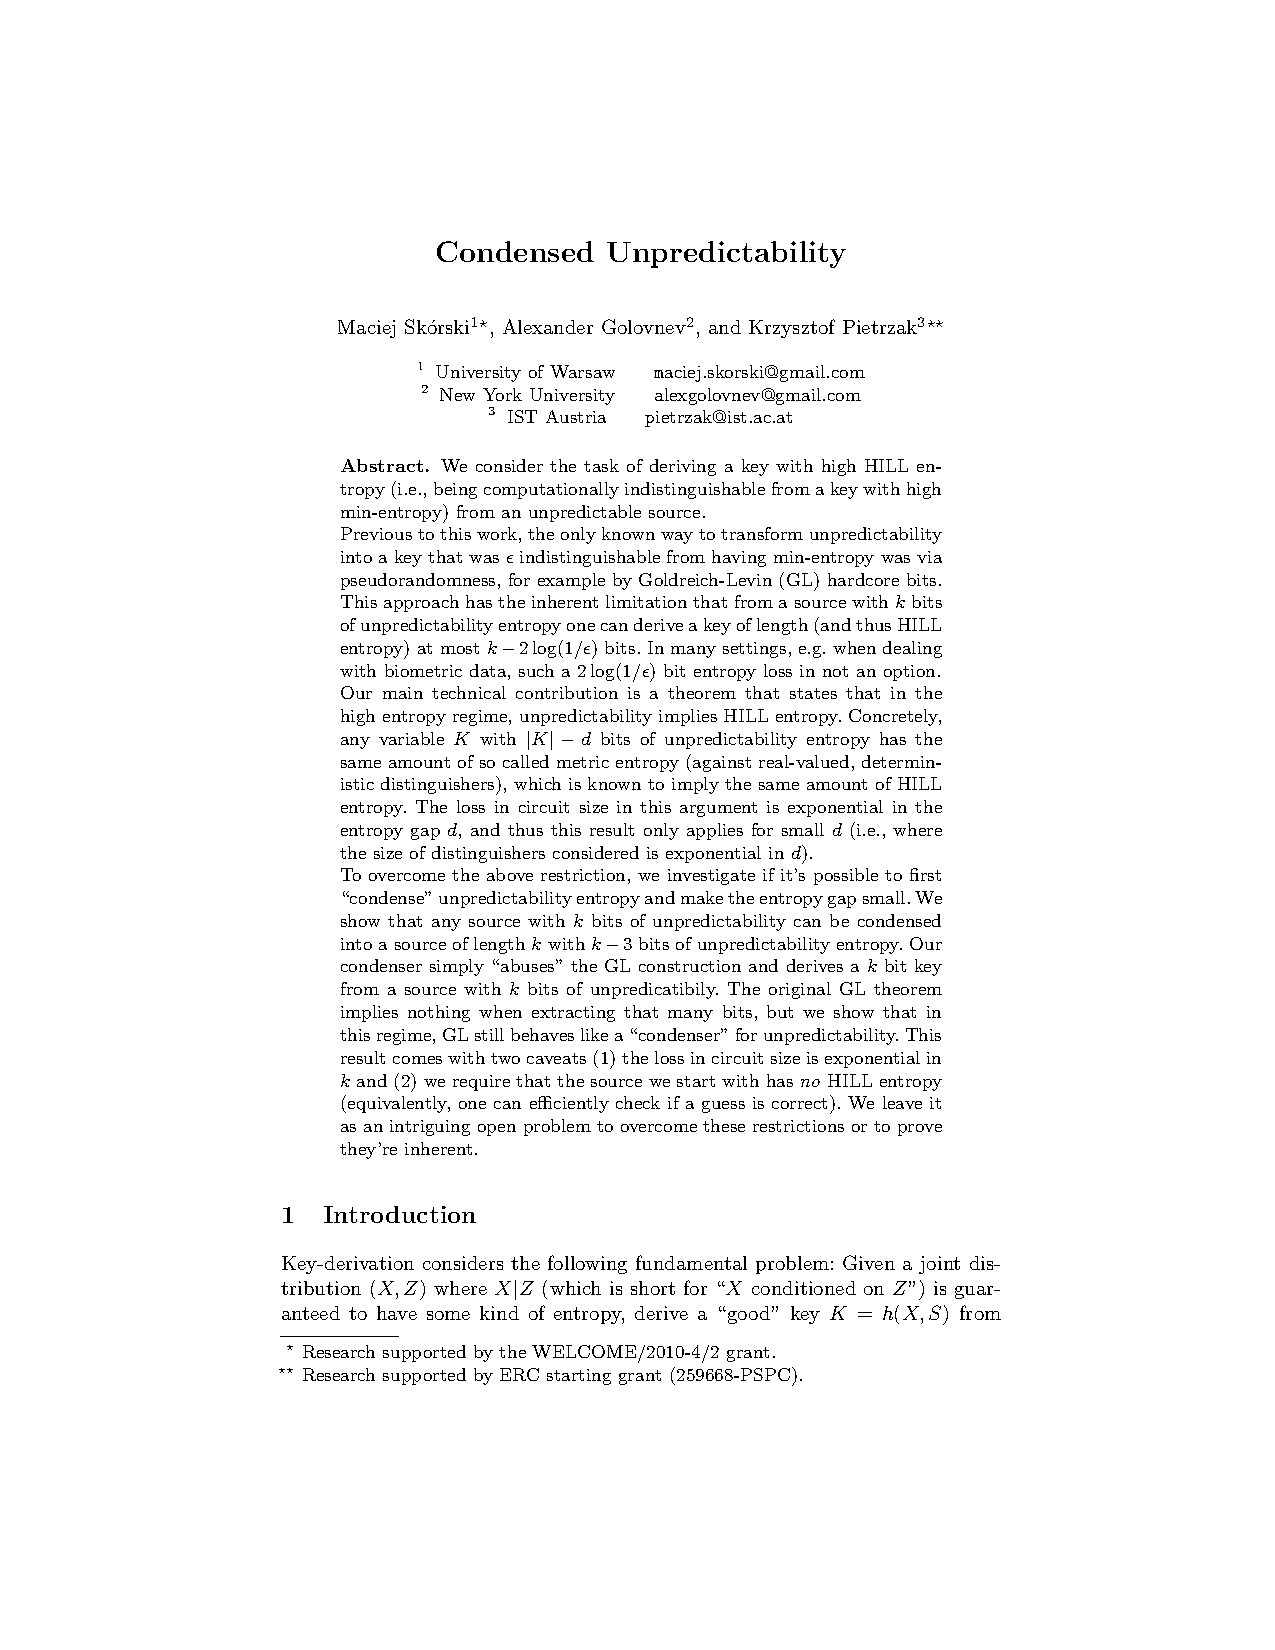
\includepdf[noautoscale, pages=-,pagecommand={}]{CondensedUnpredictability.pdf}


\chapter{Lower Bounds for Pseudoentropy Chain Rules and Transformations}
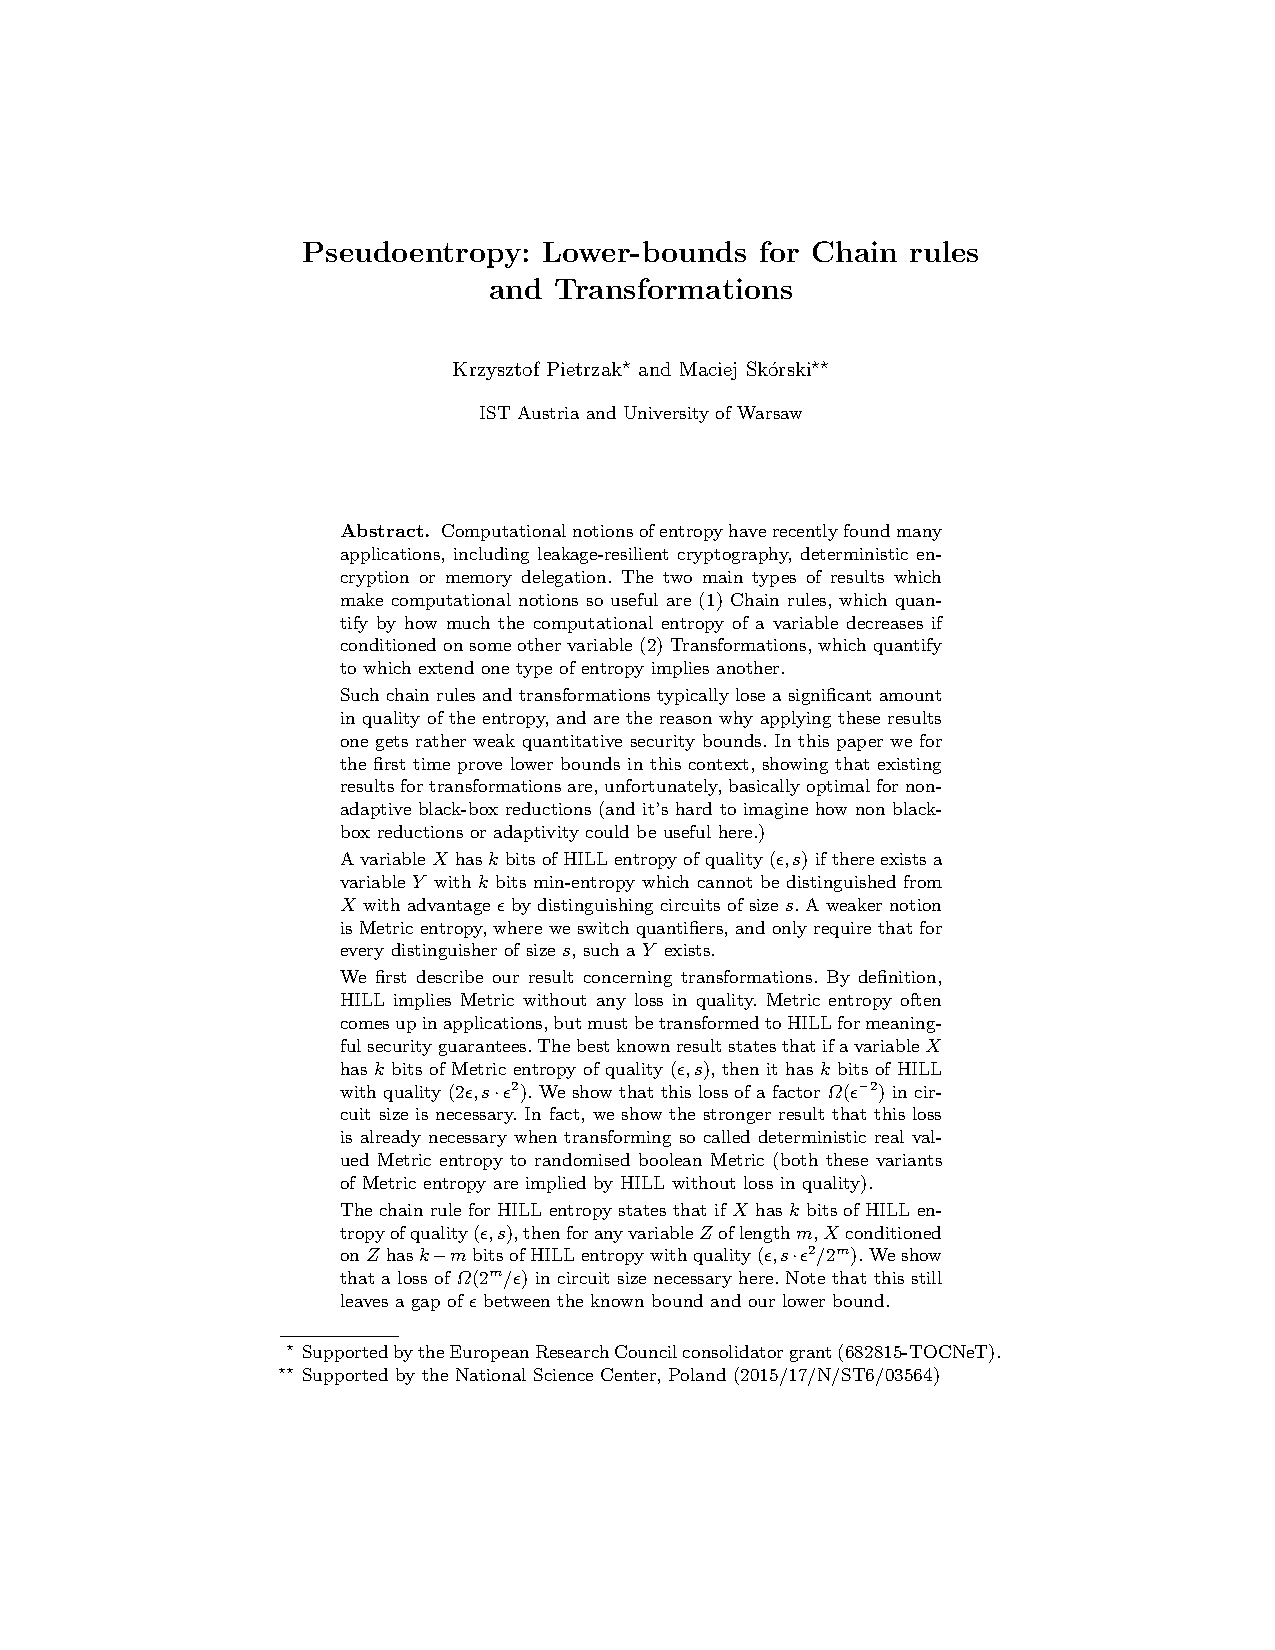
\includepdf[noautoscale, pages=-,pagecommand={}]{PseudoentropyLowerBounds.pdf}

\chapter{Simulating Auxiliary Information}
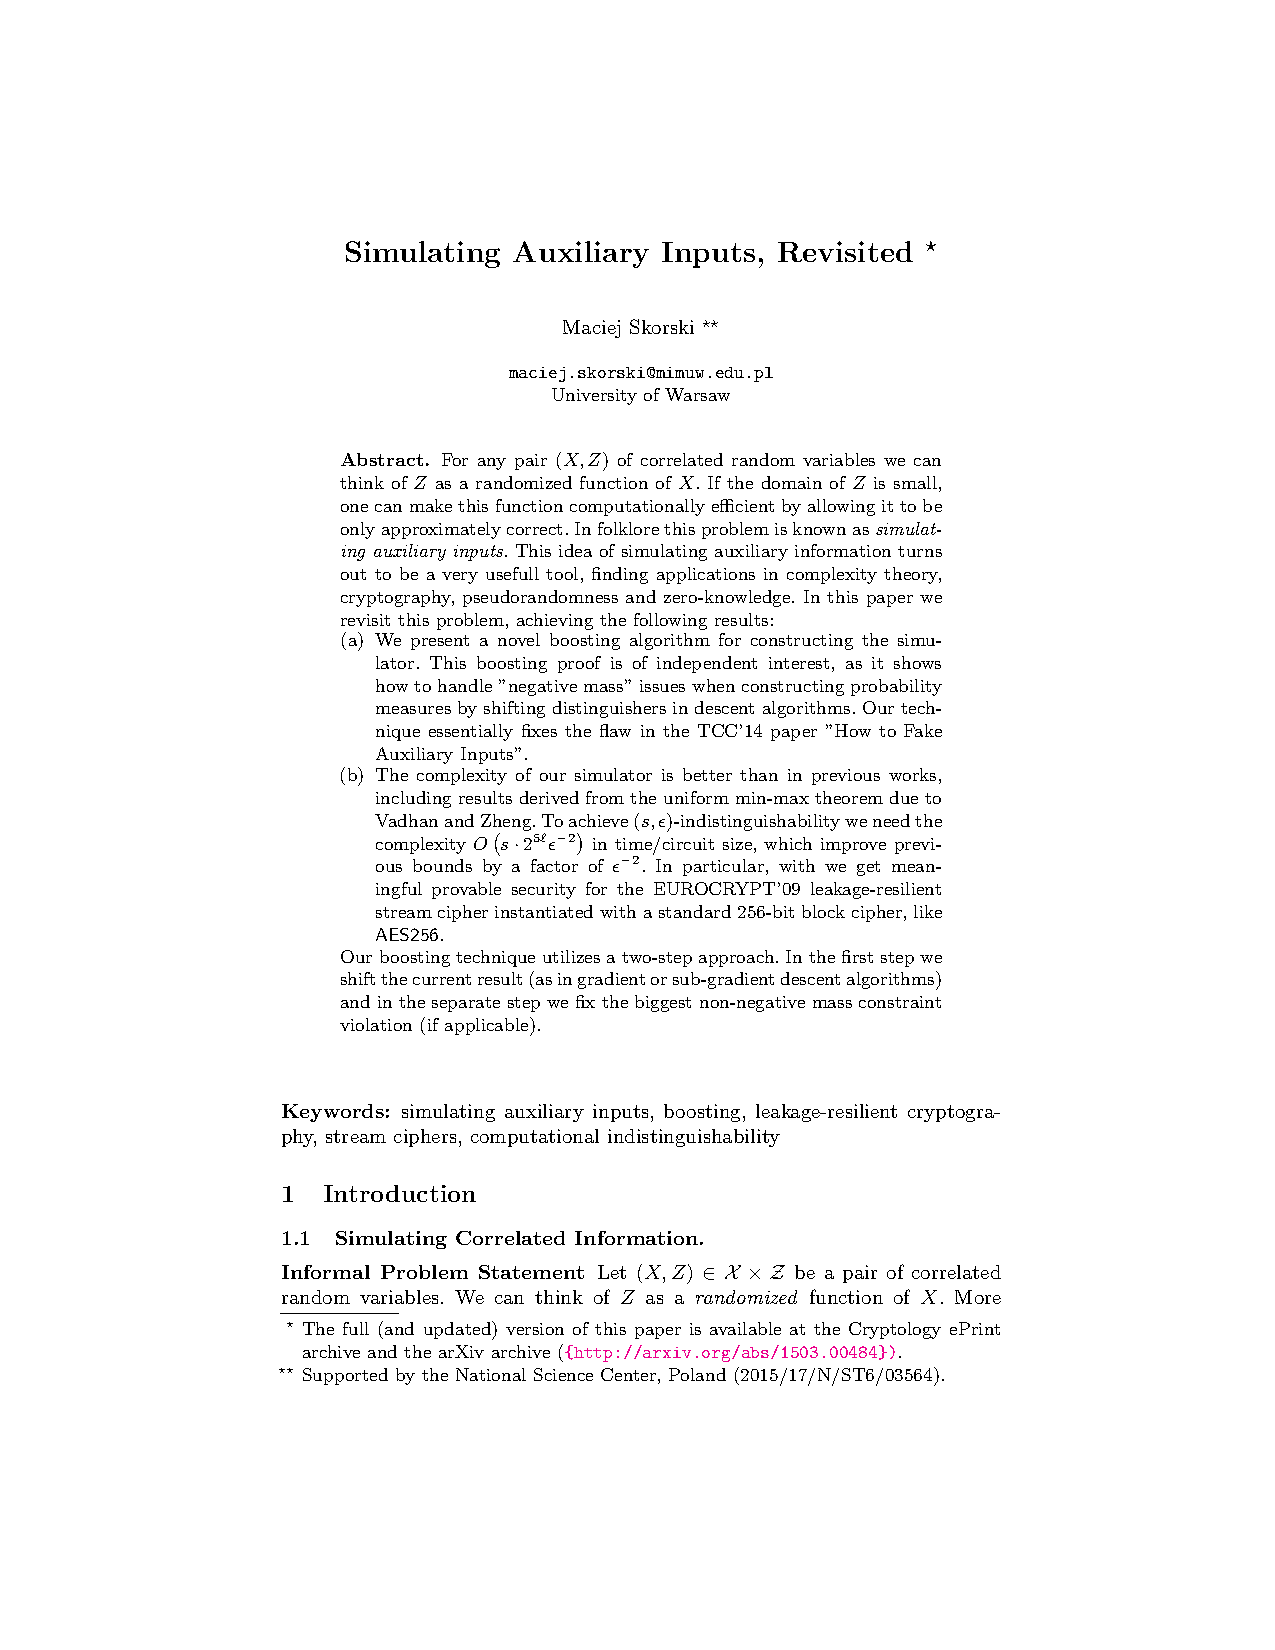
\includepdf[noautoscale, pages=-,pagecommand={}]{SimulatingAuxiliaryInformation.pdf}


\chapter{Best Generic Attacks Against Pseudoentropy}
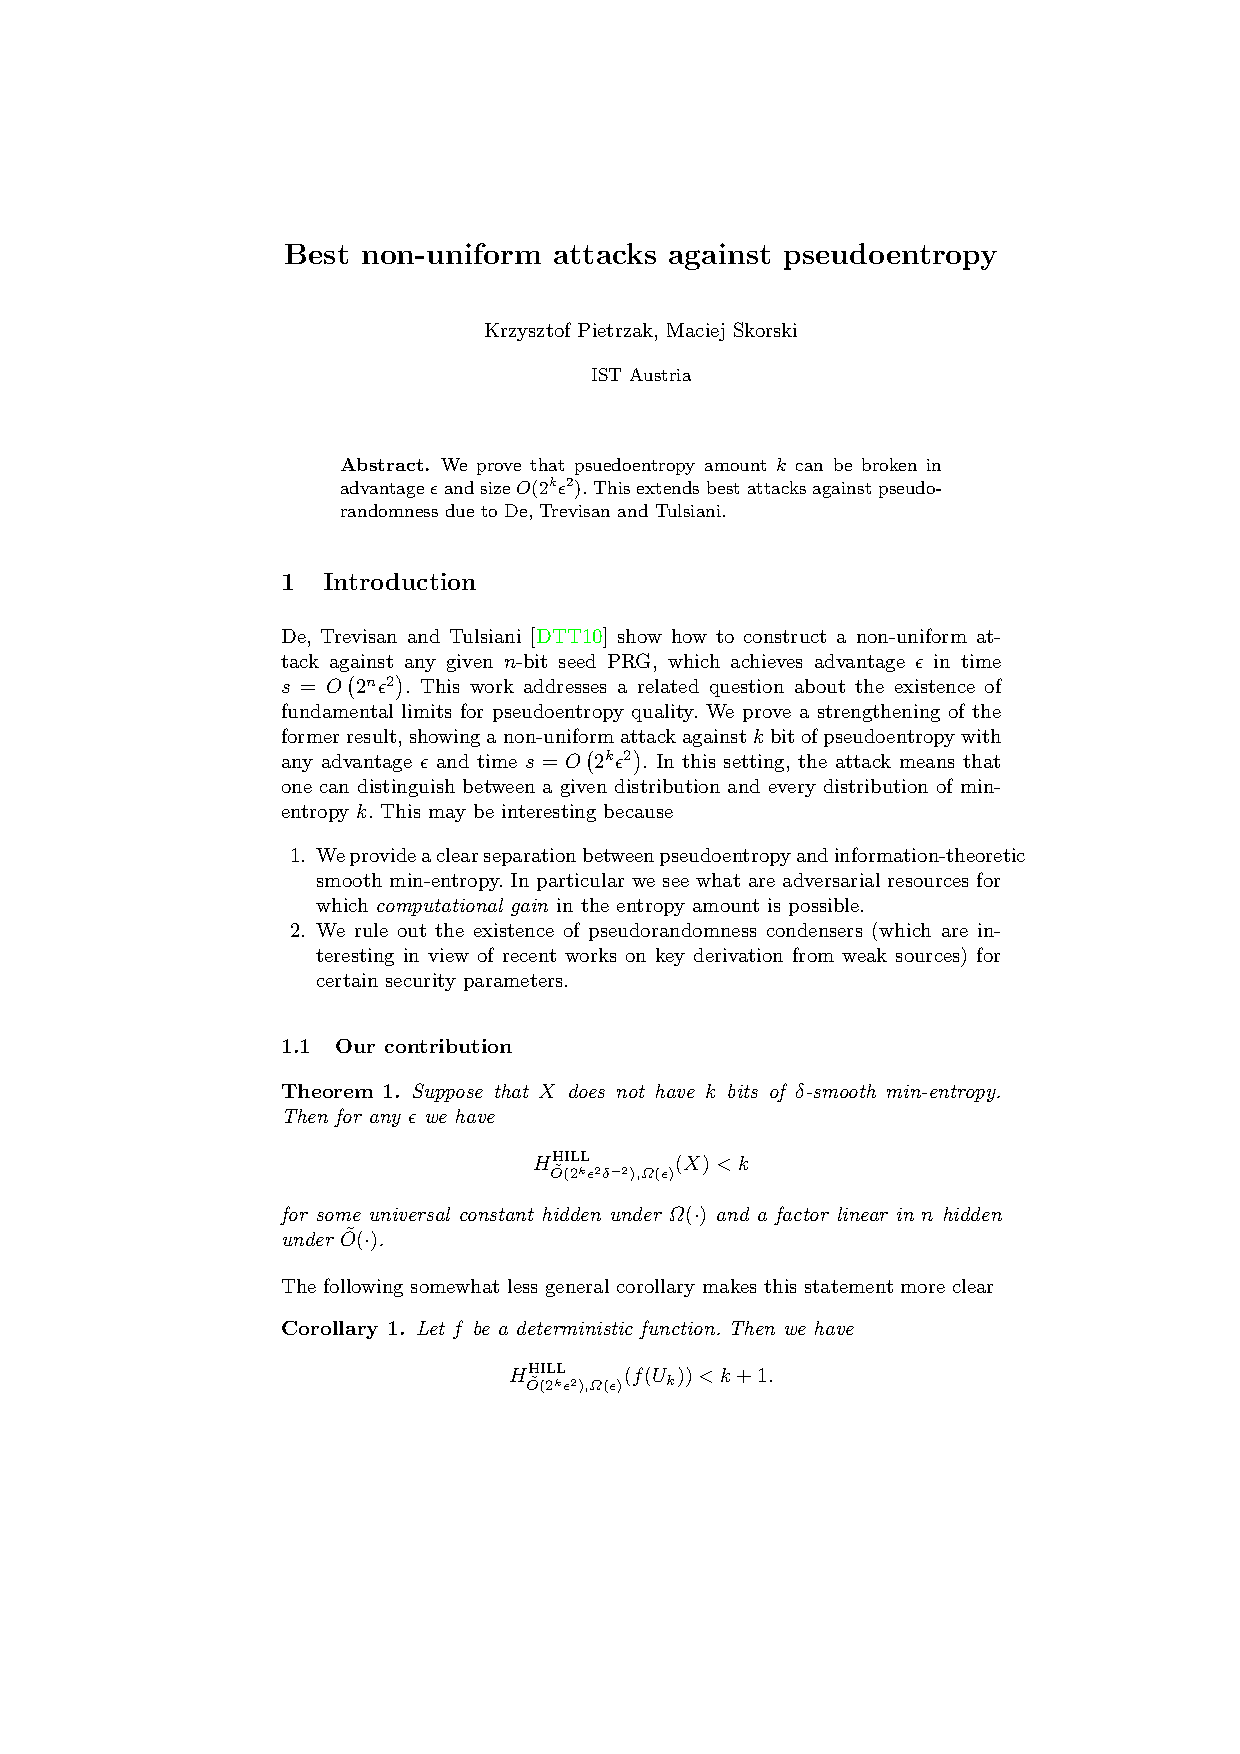
\includepdf[noautoscale, pages=-,pagecommand={}]{PseudoentropyAttacks.pdf}

\chapter{Geometric Characterization}
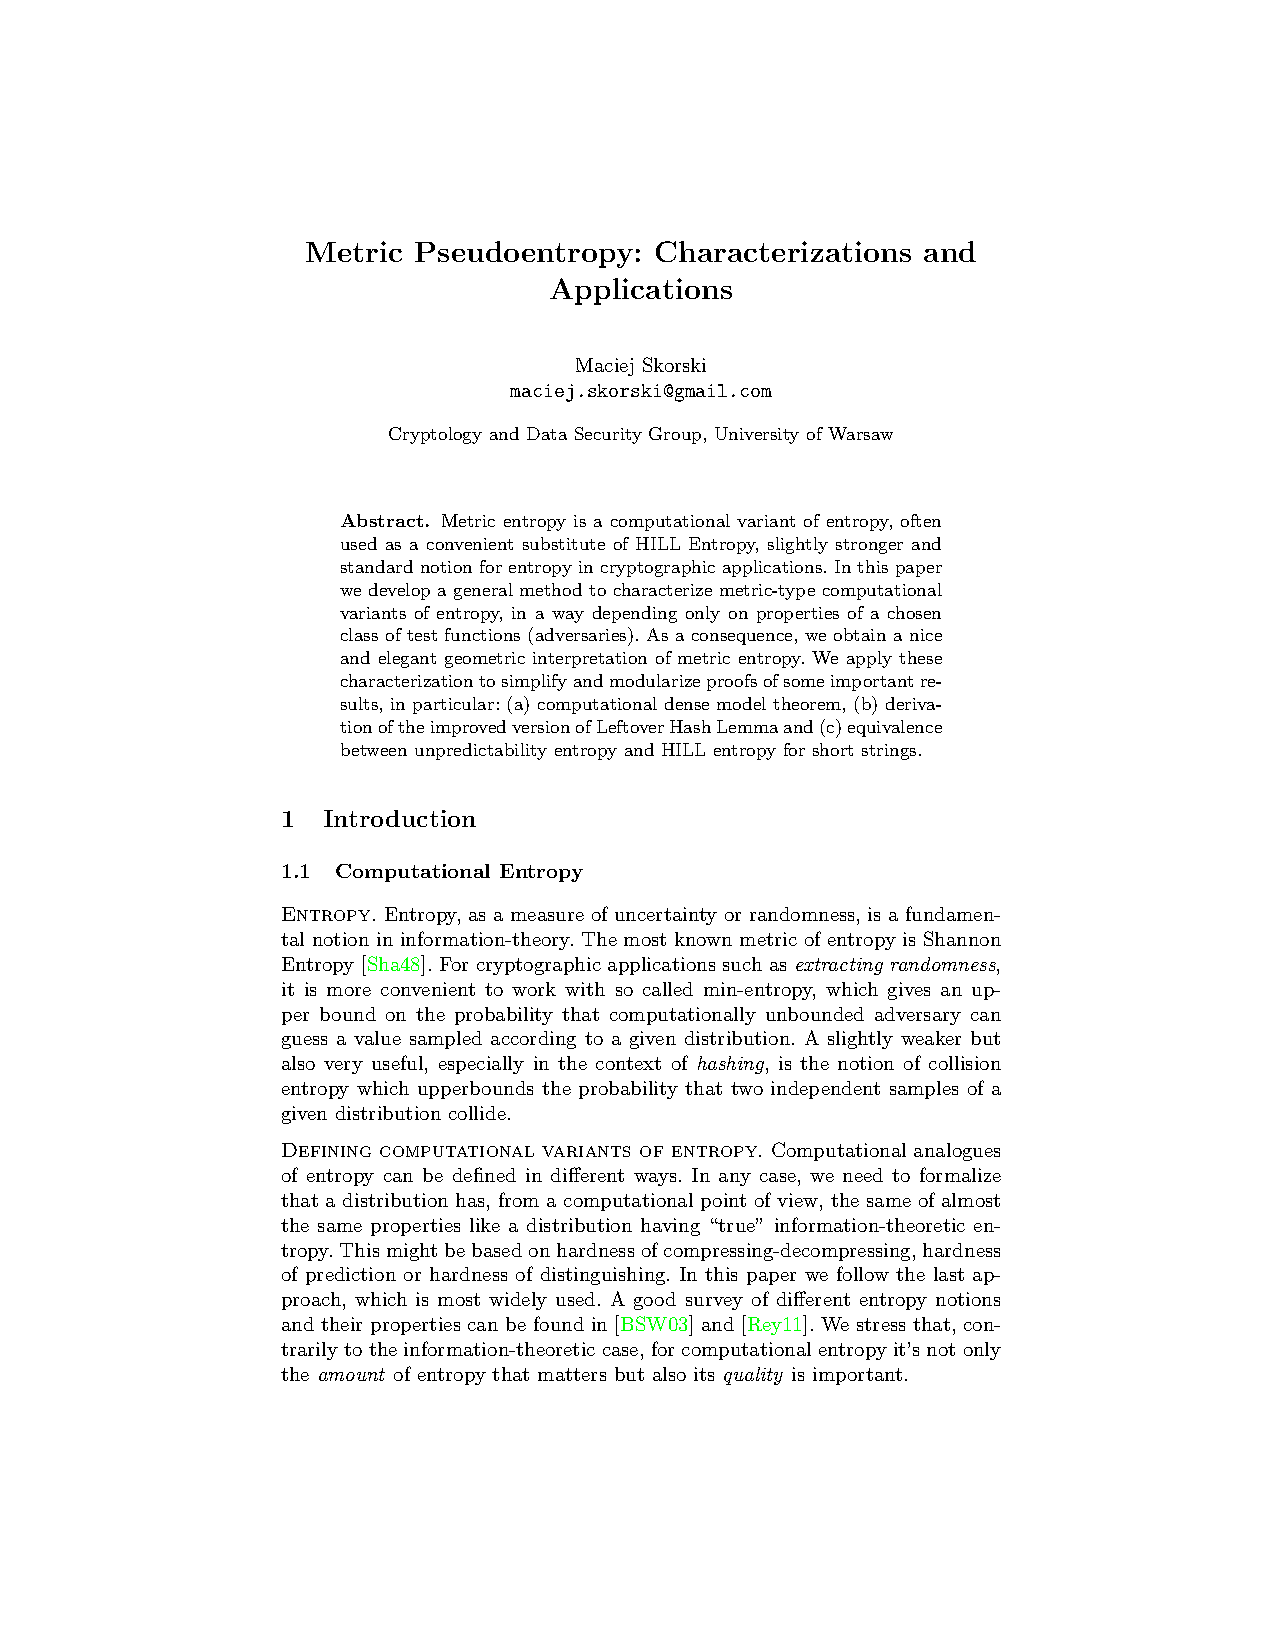
\includepdf[noautoscale, pages=-,pagecommand={}]{PseudoentropyCharacterization.pdf}


\end{document}
